% MSc Thesis of Giovanni Demasi - 987062
% Politecnico di Milano (PoliMi) - School of Industrial and Information Engineering

\documentclass{Configuration_Files/PoliMi3i_thesis}

%------------------------------------------------------------------------------
%	REQUIRED PACKAGES AND  CONFIGURATIONS
%------------------------------------------------------------------------------

% CONFIGURATIONS
\usepackage{parskip} % For paragraph layout
\usepackage{setspace} % For using single or double spacing
\usepackage{emptypage} % To insert empty pages
\usepackage{multicol} % To write in multiple columns (executive summary)
\setlength\columnsep{15pt} % Column separation in executive summary
\setlength\parindent{0pt} % Indentation
\raggedbottom

% PACKAGES FOR TITLES
\usepackage{titlesec}
% \titlespacing{\section}{left spacing}{before spacing}{after spacing}
\titlespacing{\section}{0pt}{3.3ex}{2ex}
\titlespacing{\subsection}{0pt}{3.3ex}{1.65ex}
\titlespacing{\subsubsection}{0pt}{3.3ex}{1ex}
\usepackage{color}

% PACKAGES FOR LANGUAGE AND FONT
\usepackage[english]{babel} % The document is in English  
\usepackage[utf8]{inputenc} % UTF8 encoding
\usepackage[T1]{fontenc} % Font encoding
\usepackage[11pt]{moresize} % Big fonts

% PACKAGES FOR IMAGES
\usepackage{graphicx}
\usepackage{transparent} % Enables transparent images
\usepackage{eso-pic} % For the background picture on the title page
\usepackage{subfig} % Numbered and caption subfigures using \subfloat.
\usepackage{tikz} % A package for high-quality hand-made figures.
\usetikzlibrary{}
\graphicspath{{./Images/}} % Directory of the images
\usepackage{caption} % Coloured captions
\usepackage{xcolor} % Coloured captions
\usepackage{amsthm,thmtools,xcolor} % Coloured "Theorem"
\usepackage{float}

% STANDARD MATH PACKAGES
\usepackage{amsmath}
\usepackage{amsthm}
\usepackage{amssymb}
\usepackage{amsfonts}
\usepackage{bm}
\usepackage[overload]{empheq} % For braced-style systems of equations.
\usepackage{fix-cm} % To override original LaTeX restrictions on sizes

% PACKAGES FOR TABLES
\usepackage{tabularx}
\usepackage{longtable} % Tables that can span several pages
\usepackage{colortbl}

% PACKAGES FOR ALGORITHMS (PSEUDO-CODE)
\usepackage{algorithm}
\usepackage{algorithmic}

% PACKAGES FOR REFERENCES & BIBLIOGRAPHY
\usepackage[colorlinks=true,linkcolor=black,anchorcolor=black,citecolor=black,filecolor=black,menucolor=black,runcolor=black,urlcolor=black]{hyperref} % Adds clickable links at references
\usepackage{cleveref}
\usepackage[square, numbers, sort&compress]{natbib} % Square brackets, citing references with numbers, citations sorted by appearance in the text and compressed
\bibliographystyle{abbrvnat} % I may use a different style adapted to your field

% OTHER PACKAGES
\usepackage{pdfpages} % To include a pdf file
\usepackage{afterpage}
\usepackage{lipsum} % DUMMY PACKAGE
\usepackage{fancyhdr} % For the headers
\fancyhf{}

% Input of configuration file.
% Set the geometric layout of the document
\usepackage{geometry}
\geometry{
  top=3cm,
  left = 2.0cm,
  right = 2.0cm,
  bottom=2cm,
  headheight= 2cm,
  headsep= 0cm,
}
\raggedbottom 


% Custom theorem environments
\declaretheoremstyle[
  headfont=\color{black}\normalfont\bfseries,
  bodyfont=\color{black}\normalfont\itshape,
]{colored}

\captionsetup[figure]{labelfont={color=black}} % Set colour of the captions
\captionsetup[table]{labelfont={color=black}} % Set colour of the captions
\captionsetup[algorithm]{labelfont={color=black}} % Set colour of the captions

\theoremstyle{colored}
\newtheorem{theorem}{Theorem}[section]
\newtheorem{proposition}{Proposition}[section]

% Enhances the features of the standard "table" and "tabular" environments.
\newcommand\T{\rule{0pt}{2.6ex}}
\newcommand\B{\rule[-1.2ex]{0pt}{0pt}}

% Algorithm description
\newcounter{algsubstate}
\renewcommand{\thealgsubstate}{\alph{algsubstate}}
\newenvironment{algsubstates}{
    \setcounter{algsubstate}{0}%
    \renewcommand{\STATE}{%
    \stepcounter{algsubstate}%
    \Statex {\small\thealgsubstate:}\space}
    }{}
    
% Custom theorem environment
\newcolumntype{L}[1]{>{\raggedright\let\newline\\\arraybackslash\hspace{0pt}}m{#1}}
\newcolumntype{C}[1]{>{\centering\let\newline\\\arraybackslash\hspace{0pt}}m{#1}}
\newcolumntype{R}[1]{>{\raggedleft\let\newline\\\arraybackslash\hspace{0pt}}m{#1}}

% Custom itemize environment
\setlist[itemize,1]{label=$\bullet$}
\setlist[itemize,2]{label=$\circ$}
\setlist[itemize,3]{label=$-$}
\setlist{nosep}

% Set separation of columns 
\setlength{\columnsep}{30pt}

% Create command for background pic
\newcommand\BackgroundPic{% Adding background picture
	\put(230,358){
		\parbox[b][\paperheight]{\paperwidth}{%
			\vfill
			\centering
			\transparent{0.4}
			\vfill
}}}

% Set indentation
\setlength\parindent{0pt}

% Custom title commands
\titleformat{\section}
{\color{black}\normalfont\Large\bfseries}
{\color{black}\thesection.}{1em}{}
\titlespacing*{\section}
{0pt}{2ex}{1ex}

\titleformat{\subsection}
{\color{black}\normalfont\large\bfseries}
{\color{black}\thesubsection.}{1em}{}
\titlespacing*{\subsection}
{0pt}{2ex}{1ex}

% Custom headers and footers
\pagestyle{fancy}
\fancyhf{}
      
\fancyfoot{}
\fancyfoot[C]{\thepage} % page
\renewcommand{\headrulewidth}{0mm} % headrule width
\renewcommand{\footrulewidth}{0mm} % footrule width

\makeatletter
\patchcmd{\headrule}{\hrule}{\color{black}\hrule}{}{} % headrule
\patchcmd{\footrule}{\hrule}{\color{black}\hrule}{}{} % footrule
\makeatother

% -> Create the header
\chead[C]{
\centering
\textbf{ Executive summary} \hfill \textbf{\author}
\centerline{\rule{1.0\textwidth}{0.4pt}}
}

%----------------------------------------------------------------------------
%	NEW COMMANDS DEFINED
%----------------------------------------------------------------------------

%----------------------------------------------------------------------------
%	ADDITIONAL PACKAGES
%----------------------------------------------------------------------------

%----------------------------------------------------------------------------
%	ADDITIONAL DEFINITIONS AND COMMANDS
%----------------------------------------------------------------------------

%----------------------------------------------------------------------------
%	DOCUMENT
%----------------------------------------------------------------------------

\begin{document}
    \nocite{*}

    \fancypagestyle{plain}{%
        \fancyhf{} % Clear all header and footer fields
        \fancyhead[RO,RE]{\thepage} %RO=right odd, RE=right even
        \renewcommand{\headrulewidth}{0pt}
        \renewcommand{\footrulewidth}{0pt}}

%----------------------------------------------------------------------------
%	TITLE PAGE
%----------------------------------------------------------------------------

    \pagestyle{empty} % No page numbers
    \frontmatter % Use roman page numbering style (i, ii, iii, iv...) for the preamble pages

    \puttitle{
        title=Graph Neural Network \\ Acceleration with SODA \\ Framework, % Title of the thesis
        name=Giovanni Demasi, % Author Name and Surname
        course=Computer Science and Engineering, % Study Programme
        ID  = 987062,  % Student ID number (numero di matricola)
        advisor= Prof. Fabrizio Ferrandi, % Supervisor name
        coadvisor={Serena Curzel}, % Co-Supervisor name
        academicyear={2022-23},  % Academic Year
    } % These info will be put into your Title page

%----------------------------------------------------------------------------
%	PREAMBLE PAGES: ABSTRACT (inglese e italiano), EXECUTIVE SUMMARY
%----------------------------------------------------------------------------
    \startpreamble
    \setcounter{page}{1} % Set page counter to 1

% ABSTRACT IN ENGLISH
    \chapter*{Abstract}
    Here goes the Abstract in English of your thesis followed by a list of keywords.
    The Abstract is a concise summary of the content of the thesis (single page of text)
    and a guide to the most important contributions included in your thesis.
    The Abstract is the very last thing you write.
    It should be a self-contained text and should be clear to someone who hasn't (yet) read the whole manuscript.
    The Abstract should contain the answers to the main scientific questions that have been addressed in your thesis.
    It needs to summarize the adopted motivations and the adopted methodological approach as well as the findings of your work and their relevance and impact.
    The Abstract is the part appearing in the record of your thesis inside POLITesi,
    the Digital Archive of PhD and Master Theses (Laurea Magistrale) of Politecnico di Milano.
    The Abstract will be followed by a list of four to six keywords.
    Keywords are a tool to help indexers and search engines to find relevant documents.
    To be relevant and effective, keywords must be chosen carefully.
    They should represent the content of your work and be specific to your field or sub-field.
    Keywords may be a single word or two to four words.
    \\
    \\
    \textbf{Keywords:} here, the keywords, of your thesis % Keywords

% ABSTRACT IN ITALIAN
    \chapter*{Abstract in Lingua Italiana}
    Qui va l'Abstract in lingua italiana della tesi seguito dalla lista di parole chiave.
    \\
    \\
    \textbf{Parole chiave:} qui, vanno, le parole chiave, della tesi % Keywords (italian)

%----------------------------------------------------------------------------
%	LIST OF CONTENTS/FIGURES/TABLES/SYMBOLS
%----------------------------------------------------------------------------

% TABLE OF CONTENTS
    \thispagestyle{empty}
    \tableofcontents % Table of contents
    \thispagestyle{empty}
    \cleardoublepage

%-------------------------------------------------------------------------
%	THESIS MAIN TEXT
%-------------------------------------------------------------------------
% In the main text of this thesis it is possible to write the chapters in two different ways:
%
%(1) It is possible to write:
%    \chapter{Title of the chapter}
%    *body of the chapter*
%
%(2) It is also possible to write the chapter in a separated .tex file and then include it in the main file with the following command:
%    \chapter{Title of the chapter}
%    \input{chapter_file.tex}
%
% Especially for long thesis, the second option is the recommended one.

    \addtocontents{toc}{\vspace{2em}} % Add a gap in the Contents, for aesthetics
    \mainmatter % Begin numeric (1,2,3...) page numbering

% ##########################################################################
% CHAPTER ONE - INTRODUCTION
% ##########################################################################

    \chapter{Introduction}
    \label{ch:chapter_one}%
    In recent years, deep learning has brought about a revolutionary transformation in various machine learning tasks,
spanning from image classification and video processing to speech recognition and natural language understanding.
Traditionally, these tasks have predominantly operated within the Euclidean space, where data is typically
represented.
Nevertheless, a growing number of applications now generate data from non-Euclidean domains,
presenting it in the form of complex graphs with intricate relationships and interdependencies among objects.
The inherent complexity of graph data has posed considerable challenges for existing machine learning algorithms.
Consequently, there has been a surge of studies focusing on extending deep learning techniques to accommodate
and leverage graph data.

Graph neural networks (GNNs) have been introduced in response to the growing demand for learning tasks involving
graph data, which encompasses extensive relational information among its elements.
These neural models effectively capture the interdependence among graph nodes by employing message passing mechanisms.

As Graph Neural Networks are increasingly employed, particularly in domains characterized by vast amounts of data,
such as social networks and chemistry, a need arises to optimize and accelerate their capabilities.
Inference in GNNs refers to the time the model takes to make predictions after training.
The duration of the inference process determines the speed at which queries are answered, and researchers strive to minimize this time span.

In applications of deep learning that prioritize low latency, FPGAs outperform other computing devices, such as CPUs and GPUs,
by providing superior performance.
FPGAs offer the advantage of being fine-tuned to strike the optimal balance between power efficiency and meeting performance requirements.

Due to this reason, researchers have been actively pursuing the development of new FPGA accelerators for Graph Neural Networks (GNNs) in recent times.

The conventional approach to hardware design involves a combination of manual coding and automated processing.
However, this method demands significant effort and relies heavily on the expertise of the designers, leading to varying quality of results.

To address these challenges, the objective of this thesis research study is to develop a comprehensive toolchain that, starting from PyTorch~\cite{DBLP:journals/corr/abs-1912-01703},
a cutting-edge high-level programming framework for creating neural network algorithms based on the Python programming language, enables the
automatic generation of a Graph Neural Networks (GNNs) FPGA accelerator with minimal effort required.

The suggested toolchain represents an enhancement of the SODA toolchain~\cite{9786533}.
It operates by transforming the PyTorch model, provided as input, into a multi-level intermediate representation
(MLIR)~\cite{9370308} utilizing Torch-MLIR~\cite{torch_mlir}, an MLIR based compiler toolkit for PyTorch programs.
This MLIR representation is then passed to the SODA framework to conduct hardware/software partitioning of the algorithm
specifications and architecture-independent optimizations.
Following this, the framework generates a low-level IR (LLVM IR) specifically tailored for the hardware generation engine,
PandA-Bambu~\cite{9586110}.

In pursuit of the thesis goal, various optimizations were adopted throughout the process.
Specifically, efforts were made to optimize specific computations in Graph Neural Networks during the experimental phase.
As these networks often deal with massive graph sizes, the computation time and memory requirements are substantial.
Consequently, a significant portion of the research focuses on optimizing the computation phase of Graph Neural Networks using
tailored SODA optimizations, particularly matrix multiplication.

Furthermore, limitations and challenges have been encountered along the way.
Another objective of this thesis is to analyze these limitations, ensuring they are clearly understood thoroughly.
This analysis aims to provide valuable insights for future research endeavors, enabling the development of solutions
to overcome these limitations and further enhance the proposed toolchain.

While the intended purpose of the toolchain is to be general, the experimental phase primarily focused on two specific
types of Graph Neural Networks: Graph Isomorphism Networks (GIN)~\cite{xu2019powerful} and Graph Convolutional Networks (GCN)~\cite{DBLP:journals/corr/KipfW16}.
These models were sourced from reliable GitHub implementations and were modified as necessary.

The GCN model~\cite{pygcn}, designed for node classification task and written in pure PyTorch, held particular importance for the
experimental phase as it served as the basis for the resulting accelerator.
On the other hand, the GIN model~\cite{ogb_gnn_models}, designed for graph classification task and written in PyTorch Geometric~\cite{DBLP:journals/corr/abs-1903-02428},
a library built upon PyTorch for easier development and training of Graph Neural Networks, did not progress through
the final step of the proposed toolchain.
This was due to some incompatibilities between PyTorch Geometric and Torch-MLIR, which are integral parts of this thesis research.

\section{Contributions}
\label{sec:contributions}%


\section{Thesis structure}
\label{sec:thesis_structure}%

Chapter~\ref{ch:chapter_one} introduces the context of the thesis, its objective, and its goals, including a general overview of the research's focus, contributions, and outcome.
Chapter~\ref{ch:chapter_two} presents the background needed to understand the thesis's content deeply.
In particular, it contains a summary of Graph Neural Networks, how they work, an explanation of the GNN types used in the experimental phase, and the type of tasks that they can perform, including some of their applications.
Additionally, it presents the SODA framework, an important part of this thesis's proposed toolchain.
Chapter~\ref{ch:chapter_three} instead contains an overview of the related works.
Other Graph Neural Network acceleration frameworks will be analyzed, underlying their differences compared to the research study done for this thesis and some limitations.
Chapter~\ref{ch:chapter_four} formulates the problem statement, summarizes the open issues of the research objective, and explains how the thesis goals can be helpful and their expected impact.
Chapter~\ref{ch:chapter_five} is the core chapter of the thesis, it clearly explains how the problem has been faced and what technologies have been used.
It contains a detailed description of the proposed toolchain and its working method.
Chapter~\ref{ch:chapter_six} lists all the performed experiments, gives the necessary information to reproduce them and contains their outcomes and the issues and limitations encountered.
Finally, Chapter~\ref{ch:conclusions} presents overall considerations of the study, both with the main achievements obtained and the most notable obstacles faced.
Along with this, potential improvements for future studies are considered.

% ##########################################################################
% CHAPTER TWO - BACKGROUND
% ##########################################################################


    \chapter{Background}
    \label{ch:chapter_two}%
    % The \label{...}% enables to remove the small indentation that is generated, always leave the % symbol.
    This chapter provides essential background information to enhance understanding of the thesis content and objectives.
It begins by introducing the graph data structure, which is crucial for comprehending Graph Neural Networks.
Additionally, the chapter provides an introduction to Graph Neural Networks, outlining their capabilities and exploring various applications.
Furthermore, it introduces two essential tools, SODA and Bambu, which are integral parts of the SODA Toolchain that served as the foundation for this research study.

\section{Graphs}
\label{sh:graphs}%

\textit{Graphs} are a data structure representing a collection of objects, known as vertices or nodes, and a set of edges~\cite{DBLP:journals/corr/abs-1812-08434}.
In a graph, the edges can be either directed or undirected, as shown in Figure~\ref{fig:directed_vs_undirected}, and they typically connect two vertices, which may or may not be distinct.
The vertices represent entities or elements, and the edges represent their relationships or connections.

\begin{figure}[b]
    \centering
    \subfloat[Directed Graph\label{fig:directed_graph}]{
        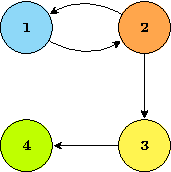
\includegraphics[width=0.2\textwidth]{Images/directed_graph}
    }
    %\quad
    \hspace{0.15\textwidth}
    \subfloat[Undirected Graph\label{fig:undirected_graph}]{
        \captionsetup{width=.4\textwidth}
        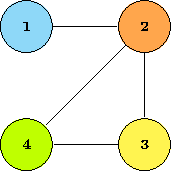
\includegraphics[width=0.2\textwidth]{Images/undirected_graph}
    }
    %\caption[Shorter caption]{This is a very long caption you don't want to appear in the List of Figures.}
    \caption{Example of directed and undirected graphs}
    \label{fig:directed_vs_undirected}
\end{figure}

Graphs serve as a versatile tool for describing diverse forms of data.
Molecules, the fundamental units of matter, are composed of atoms and electrons arranged in three-dimensional space.
In this intricate structure, all particles interact with each other.
However, when a pair of atoms are stably positioned at a specific distance, we refer to their connection as a covalent bond.
These bonds with distinct atomic distances can vary in nature, such as single or double bonds.
Representing this complex three-dimensional object as a graph offers a practical and widely adopted abstraction, where atoms are nodes and covalent bonds act as edges~\cite{DBLP:journals/corr/DuvenaudMAGHAA15}.

Social networks provide another domain where graphs find utility.
They serve as valuable tools for examining patterns within the collective behavior of people, institutions, and organizations.
By representing individuals as nodes and their relationships as edges, we can construct a graph that effectively captures groups of people and their interconnectedness.

\subsection{Graph Representation}
\label{subsec:graph_representation}

Here I am going to talk about how graphs can be represented.
Especially the ways encountered during the research: adjacency matrix, COO and CSR.

%TODO: add an image with a graph and its representation in the 3 different format

\section{Graph Neural Networks}
\label{sh:graph_neural_networks}%

%TODO: add an example image of a GNN

Graph neural networks (GNNs) are deep learning techniques that operate on graph-structured data.
Thanks to their impressive performance, GNNs have recently gained significant popularity as a widely adopted method for graph analysis.

Graph Neural Networks (GNNs) are designed to process graph data and consist of multiple interconnected layers.
At its core, a GNN is an algorithm that exploits the connectivity within a graph to understand and represent the relationships between nodes.
By relying on the graph's structure, the GNN iteratively processes input edge, vertex, and graph feature vectors, which encode known attributes and transforms them into output feature vectors that capture the desired predictions.
Each Graph Neural Network typically encompasses three main stages: pre-processing, iterative updates and decoding or readout~\cite{DBLP:journals/corr/abs-2010-00130}.
\begin{enumerate}
    \item \textbf{Pre-processing}: this initial step, while optional, involves transforming the input feature vectors and graph structure representation through a pre-processing procedure.
    \item \textbf{Iterative updates}: following pre-processing, the feature vectors of each edge and vertex undergo iterative updates using aggregate-combine functions.
          For edge updates, attributes from the edge itself, connected vertices, and the graph are aggregated and combined to generate a new edge feature vector.
          Similarly, vertex updates involve aggregating feature vectors from neighboring vertices $\mathcal{N}(v)$ and combining them to obtain a new feature vector.
          This iterative process gradually incorporates relationships between increasingly distant nodes and edges, allowing for multi-hop updates.
          Furthermore, the graph may coarsen through pooling~\cite{DBLP:journals/corr/abs-1806-08804} (i.e. selective reduction or adjustment of either the graph structure or the neighborhood set of each node) in each subsequent layer, or the neighborhood set may change via layer sampling~\cite{DBLP:journals/corr/HamiltonYL17} (i.e. coarsening the graph from one layer to the next, leading to a reduction in the number of nodes that need to be processed during aggregation and combination steps).
    \item \textbf{Decoding or readout}: once the graph possesses a global feature vector, it is updated once upon completion of edge and node updates.
          The final output can be an edge/node embedding, representing specific information about each edge or node in a low-dimensional feature vector format, or a graph embedding that summarizes the entire output graph.
\end{enumerate}
Performing these stages on large and sparse graphs can introduce dynamic computational data flow and numerous irregular memory access patterns.

Similar to other neural networks, the processing of a GNN is influenced by its architecture.
GNNs, as previously said, are structured into layers, each representing an iteration in the update process described earlier.
This layering allows information to propagate across nodes, enabling the influence of distant nodes.
Consequently, the appropriate number of layers in a GNN will vary depending on the significance of relationships among distant nodes in a specific application.
The commonly adopted range for the number of GNN layers is 1 to 5, as an excessive number of layers can introduce undesired problems such as feature over-smoothing, vanishing gradients, or over-fitting~\cite{DBLP:journals/corr/abs-1801-07606}.

Graph Neural Networks are a group of neural networks which are designed to solve different tasks.
Prediction tasks on graphs can generally be classified into three categories: graph-level, node-level, and edge-level predictions~\cite{sanchez-lengeling2021a}.

In a graph-level task, the objective is to predict the property or characteristic of an entire graph.
For instance, when considering a molecule represented as a graph, we might aim to predict attributes such as its likelihood of binding to a receptor associated with a specific disease.
This assignment is comparable to image classification tasks, where the objective is to assign a label to an entire image.
Similarly, in text analysis, sentiment analysis serves as a similar problem where the goal is to determine a complete sentence's overall mood or emotion in one go.

Node-level tasks involve predicting the identity or function of individual nodes within a graph.
One example of a node-level task is node classification in a social network.
Given a social network graph where nodes represent individuals and edges represent relationships between them, the task is to predict the demographic attributes or characteristics (e.g., age, gender, occupation) of each node based on their connection patterns and features.
Drawing an analogy to image processing, node-level prediction problems can be compared to image segmentation tasks, where the objective is to assign labels to each pixel in an image based on its role.
Similarly, in text analysis, a comparable task would involve predicting the parts of speech for each word in a sentence, such as identifying whether a word is a noun, verb, adverb, and so on.


The remaining prediction task in graphs pertains to edge prediction.
One example of an edge-level task is link prediction in a social network.
Given a graph representing a social network where, as before, in node-level tasks, nodes correspond to individuals and edges represent relationships between them, the edge-level task aims to predict missing or potential connections between nodes.
This can involve predicting the likelihood of a future friendship or the probability of a collaboration between individuals based on their shared characteristics or mutual connections in the network.

Different popular Graph Neural Network architectures have been proposed recently, some of which are more suitable for some tasks than others.
A summary of two types of GNNs used in the experimental phase is provided in the following sections.

\subsection{Graph Convolutional Network}
\label{subsec:graph_convolutional_network}%

A graph convolutional network (GCN)~\cite{DBLP:journals/corr/KipfW16, daigavane2021understanding} is a type of neural network architecture explicitly designed to operate on graph-structured data.
GCNs aim to learn node representations by aggregating and combining information from neighboring nodes in the graph.
The core idea behind GCNs is to perform convolution-like operations on the graph, where the convolutional filters are defined based on the graph's adjacency matrix or other graph-specific structures.
This enables GCNs to capture and leverage the structural information encoded in the graph to make predictions or perform downstream tasks.
GCNs have demonstrated effectiveness in various applications, including node classification, link prediction, and graph classification.

Given an undirected graph $\mathcal{G} = (V, E)$, where $V$ represents the set of nodes (vertices), and $E$ represents the set of edges, with an adjacency matrix $\tilde{A}=A+I_N$, where $I_N$ is the identity matrix, the layer-wise propagation rule in a GCN can be expressed as:
\begin{equation}
    \label{eq:gcn_convolution}
    H^{(l+1)} = f(\tilde{D}^{-\tfrac{1}{2}}  \tilde{A}  \tilde{D}^{-\tfrac{1}{2}}  H^{(l)}  W^{(l)})
\end{equation}

Where $H^{(l)} \in \mathbb{R}^{N \times D}$ is the input node features matrix, $W^{(l)}$ is a layer-specific learnable weight matrix, $\tilde{D}$ is the degree matrix defined as $\tilde{D}_{ii} = \sum_{j} \tilde{A}_{ij}$, and $f(\cdot)$ represents a non-linear activation function applied element-wise, such as $ReLU(\cdot) = max(0, \cdot)$.
The equation above demonstrates the propagation of node features through graph convolution, where the adjacency matrix $\tilde{A}$ captures the connectivity information of the graph, $\tilde{D}^{-\tfrac{1}{2}}$ normalizes the adjacency matrix, and $H^{(l)}  W^{(l)}$ performs a linear transformation of node features.
The resulting $H^{(l+1)}$ represents the updated node representations after the graph convolution operation.
In practice, multiple graph convolutional layers can be stacked to capture increasingly complex relationships and refine the node representations further.

\subsection{Graph Isomorphism Network}
\label{subsec:graph_isomorphism_network}%

A Graph Isomorphism Network (GIN)~\cite{xu2019powerful, daigavane2021understanding} is a type of neural network architecture designed to operate on graph-structured data by capturing graph isomorphism, which is the property of two graphs having the same structure, inspired by the Weisfeiler-Lehman (WL) graph isomorphism test~\cite{xu2019powerful}.
GINs aim to learn node representations that are invariant under graph isomorphism, enabling them to generalize across different graphs with similar structures.

The learned vertex features from GIN-Conv can be directly utilized for tasks such as node classification and link prediction. It is possible to perform this model as:
\begin{equation}
    \label{eq:gin_function}
    h_v^{(k+1)} = MLP^{(k)} \left( \left( 1 + \epsilon^{(k)} \right) \cdot h_v^{(k)} + \sum_{u \in \mathcal{N}(v)} h_u^{(k)} \right)
\end{equation}

Where $h_v^{(k)}$ represents the initial node representation of node $v$, $\mathcal{N}(v)$ represents the neighborhood of node $v$, $\epsilon$ is a learnable
parameter or a fixed scalar, $MLP( \cdot )$ represents a Multi Layer Perceptron and $h_v^{(k+1)}$ represents the updated node representations.

In the neighborhood aggregation process of GINs, each node's representation is updated by considering its own representation and its neighbors' representations.
The neighborhood aggregation is performed through the MLP operation, followed by non-linear activation.

GINs are trained using graph-level objectives, such as graph classification or property prediction, and aim to learn invariant representations under graph isomorphism, allowing them to generalize well to unseen graphs with similar structures.
However, even if the node embeddings acquired through GIN can be directly applied to tasks such as node classification and link prediction, in the case of graph classification tasks, it is necessary to use a Readout function that takes individual node embeddings as input and produces the embedding representation for the entire graph.

The Readout function is then utilized to generate the overall representation of the graph, leveraging the individual vertex representations.
By concatenating the results from all iterations of GINConv, the final graph representation is obtained as:
\begin{equation}
    \label{eq:gin_readout}
    h_G = CONCAT \left( READOUT \left( \left\{ h_v^{(k)} | v \in G \right\} \right) | k = 0, 1, ..., K \right)
\end{equation}

Where $READOUT$ in~\ref{eq:gin_function} can be replaced with a sum operator in order to generalize the WL test~\cite{xu2019powerful}.


\section{SODA Toolchain}
\label{sh:soda}%

SODA~\cite{9786533} is a software-defined accelerator synthesizer.
It enables the creation of highly specialized accelerators from algorithms designed in high-level programming frameworks.
The synthesizer comprises a compiler-based frontend that interfaces with high-level programming frameworks, applying advanced optimizations.
It also includes a compiler-based backend responsible for generating Verilog code and interfacing with external tools to compile the final design, which can be applied to application-specific integrated circuits (ASICs) or field-programmable gate arrays (FPGAs).

SODA's exceptional power lies in its ability to offer a fully automated end-to-end hardware compiler, eliminating the need for human intervention and any modifications to the input code.
The SODA synthesizer framework comprises two main components: a compiler-based frontend and a compiler-based hardware generation engine.
This framework seamlessly integrates with high-level Python frameworks by accepting their input descriptions, which are then translated by the frontend into a high-level intermediate representation (IR).
Leveraging the multi-level intermediate representation (MLIR), the frontend facilitates hardware/software partitioning of algorithm specifications and performs architecture-independent optimizations.
Following this, it generates a low-level IR (LLVM IR) that is utilized by the hardware generation engine, PandA-Bambu~\cite{9586110}.
PandA-Bambu can accept LLVM IR as input, making it a cutting-edge open-source HLS tool.
Throughout the entire SODA toolchain, compiler passes are employed to implement optimizations at all levels, greatly influencing the generated hardware designs' performance, area, and power characteristics.

\subsection{SODA-OPT Frontend}
\label{subsec:soda_frontend}%

SODA-OPT, the high-level compiler frontend of the SODA synthesizer, performs search, outlining, optimization, dispatching, and acceleration pass on the input program.
Its primary objective is to prepare the program for hardware synthesis, targeting either FPGAs or ASICs.
To accomplish these tasks, SODA-OPT relies on and extends the MLIR framework.
MLIR is a framework that facilitates the development of reusable, extensible, and modular compiler infrastructure by defining dialects.
These dialects serve as self-contained intermediate representations (IRs) that adhere to the meta-IR syntax of MLIR.
By utilizing dialects, code can be modeled at different levels of abstraction, allowing for specialized representations that aid in specific compiler optimizations.

 Code regions selected for hardware acceleration undergo an optimization pipeline that progressively lowers them through various MLIR dialects until they are ultimately translated into an LLVM IR format tailored explicitly for hardware synthesis.
On the other hand, the host module is lowered into an LLVM IR file containing runtime calls to control the generated custom accelerators.

\subsection{SODA Synthesizer Frontend}
\label{subsec:soda_backend}%

Bambu, the SODA synthesizer backend, harnesses cutting-edge HLS techniques to produce accelerator designs using the low-level LLVM IR generated by the SODA frontend.
Bambu boasts multiple frontends based on standard compilers such as GCC or CLANG.
It constructs an internal IR to execute HLS steps and generates designs in HDL formats, such as Verilog or VHDL.
In addition to synthesizable HDL, Bambu can automatically generate testbenches for verification purposes.
Using Bambu, the SODA synthesizer can target both FPGAs and ASICs.

Bambu is optimized to handle a broad range of C and C++ constructs while also being able to process LLVM IR through its internal Clang frontend.
Through SODA-OPT, Bambu can be connected with MLIR code.
The LLVM IR generated after SODA-OPT's high-level optimizations undergoes explicit restructuring for HLS, resulting in more efficient accelerators than direct translation from MLIR to LLVM IR.

Bambu generates designs at the Register Transfer Level (RTL), adhering to the Finite State Machine with Datapath (FSMD) model.
These generated accelerators can subsequently be integrated into larger system-level designs, with or without microcontrollers controlling the execution.


% ##########################################################################
% CHAPTER THREE - RELATED WORK
% ##########################################################################


    \chapter{Related Work}
    \label{ch:chapter_three}%
    Accelerating Graph Neural Networks (GNNs) has become a subject of intense interest within the research community, encompassing the exploration of ASIC and FPGA accelerators.
In this chapter, a comprehensive examination is conducted on cutting-edge Graph Neural Networks FPGA accelerators and design flows based on High-Level Synthesis (HLS).
As explained in Chapter 6, particular emphasis has been placed on optimizing matrix-matrix multiplication during this thesis research study.
Consequently, this chapter also delves into the relevant literature concerning various approaches to Matmul optimization.

\section{Chapter structure}
\label{sh:related_work_structure}


\section{Software frameworks}
\label{sh:related_work_software_frameworks}

The challenges posed by GNN processing have led to inefficiencies in traditional deep neural network (DNN) libraries and graph processing frameworks.
This is primarily due to the alternating computational phases characteristic of GNNs.
While DNN libraries excel in accelerating combination operations within vertices and edges, they need help with aggregation tasks.
On the other hand, graph processing libraries effectively handle irregular memory accesses during graph traversal but assume simplistic operations at the vertices, which is not the case in GNNs. Recent research studies tried to bridge the gap by adapting the DNN libraries to overcome Graph Neural Network challenges.

The two main software frameworks trying to accelerate Graph Neural Networks computation are PyTorch Geometric~\cite{DBLP:journals/corr/abs-1903-02428} and Deep Graph Library~\cite{DBLP:journals/corr/abs-1909-01315}.
They both provide a lot of examples and code for multiple GNN architectures providing optimizations that could work for the acceleration of both training and inference.

PyTorch Geometric is a PyTorch-based library specifically designed for deep learning on input data with irregular structures, including graphs, point clouds, and manifolds.
In addition to offering comprehensive graph data structures and processing techniques, it incorporates many state-of-the-art methods from relational learning and 3D data processing domains.
PyTorch Geometric achieves remarkable data throughput by introducing efficient handling of mini-batches containing input examples of varying sizes and efficiently handling sparsity through specialized GPU scatter and gather kernels, which operate on all edges and nodes concurrently, as opposed to relying on sparse matrix multiplication kernels.
A key aspect of PyG involves defining a message-passing interface encompassing message and update functions for neighborhood aggregation and combination and multiple pooling operations.

DGL is a recently developed library that seamlessly integrates with TensorFlow, PyTorch, or MXNet.
It introduces three essential functions: message for aggregating edges, update and reduce for aggregating and combining at the nodes.
DGL adopts a matrix multiplication approach to enhance performance and harnesses specialized kernels designed for GPUs or TPUs.
Specifically, both sampled dense-dense and sparse matrix multiplications and options for node, edge, or feature parallelization are considered.
DGL intelligently selects the optimal parallelization scheme using heuristics, considering various factors, including the input graph.
It distills the computational patterns of GNNs into a set of generalized sparse tensor operations, which facilitate extensive parallelization.
By prioritizing the graph as the central programming abstraction, DGL enables transparent optimizations.
Furthermore, through a framework-neutral design philosophy, DGL allows users to effortlessly port and leverage existing components across multiple deep learning frameworks.

The approach used by DGL outperformed PyTorch Geometric in training Graph Neural Networks, as stated in their paper~\cite{DBLP:journals/corr/abs-1909-01315}.
However, both libraries target CPU and GPU architectures.
Knowing the extreme computational power of FPGA, the field of hardware accelerators started gaining more and more interest, with the expectation of having GNN hardware accelerators capable of outperforming the performance of CPU-GPU targeting libraries.




% ##########################################################################
% CHAPTER FOUR - PROBLEM FORMULATION
% ##########################################################################


    \chapter{Problem Formulation}
    \label{ch:chapter_four}%

    Problem formulated in a clear way, what we did and how, with open issues and thesis goals.

% ##########################################################################
% CHAPTER FIVE - TOOLCHAIN
% ##########################################################################


    \chapter{FPGA Toolchain for Graph Neural Network Acceleration}
    \label{ch:chapter_five}%

    Introduction of the way I faced the problem, with the motivation for the followed approach.
    Explanation of the toolchain in a clear way.

% ##########################################################################
% CHAPTER SIX - EXPERIMENTAL RESULTS
% ##########################################################################


    \chapter{Experimental Results}
    \label{ch:chapter_six}%

    Chapter dedicated to the outcome of the results, what I have obtained and what limitations have been encountered.
    Explaining the still open issues and research suggestions.



% ##########################################################################
% CHAPTER SEVEN - CONCLUSION
% ##########################################################################

    \chapter{Conclusions and Future Developments}
    \label{ch:conclusions}%
    Final chapter containing the main conclusions of my research
    and possible future developments.

%##########################################################################
%	BIBLIOGRAPHY
%##########################################################################

    \addtocontents{toc}{\vspace{2em}} % Add a gap in the Contents, for aesthetics
    \bibliography{Thesis_bibliography} % The references information are stored in the file named "Thesis_bibliography.bib"

%-------------------------------------------------------------------------
%	APPENDICES
%-------------------------------------------------------------------------

    \cleardoublepage
    \addtocontents{toc}{\vspace{2em}} % Add a gap in the Contents, for aesthetics
    \appendix

%
%    \chapter{Appendix A}
%    If you need to include an appendix to support the research in your thesis, you can place it at the end of the manuscript.
%    An appendix contains supplementary material (figures, tables, data, codes, mathematical proofs, surveys, \dots)
%    which supplement the main results contained in the previous chapters.
%
%
%    \chapter{Appendix B}
%    It may be necessary to include another appendix to better organize the presentation of supplementary material.

% LIST OF FIGURES
    \listoffigures

% LIST OF TABLES
    \listoftables

% LIST OF SYMBOLS
% Write out the List of Symbols in this page
    \chapter*{List of Symbols} % You have to include a chapter for your list of symbols (
    \begin{table}[H]
        \centering
        \begin{tabular}{lll}
            \textbf{Notation} & \textbf{Description} \\\hline\\[-9px]
            $\mathcal{G} = (V, E)$        & The input graph for the GNN  \\[2px]
            $V$ & Set of vertices of the graph \\[2px]
            $E$ & Set of edges of the graph \\[2px]
            $\mathcal{N}(v)$ & Set of neighbors of vertex $v$ \\[2px]
            $A \in \mathbb{R}^{N \times N}$        & Adjacency matrix of $\mathcal{G}$ ($N$ : number of nodes)  \\[2px]
            $\tilde{D}$ & Degree matrix of the graph \\[2px]
            $W^{(l)}$ & Weight matrix of the neural network ($l$ : layer) \\[2px]
            $H^{(l)}$ & Input node features matrix ($l$ : layer) \\[2px]
            $h_v$ & Node representation of node $v$ \\[2px]
            $\epsilon$ & Learnable parameter or fixed scalar \\[2px]
            $I$ & Identity matrix \\[2px]

        \end{tabular}\label{tab:symbols_table}
    \end{table}

% ACKNOWLEDGEMENTS
    \chapter*{Acknowledgements}
    Acknowledgements here...

    \cleardoublepage

\end{document}
